% ------------------------------------------------------------------------------
% TYPO3 CMS 7.2 - What's New (English Version)
%
% @author	Michael Schams <schams.net>
% @license	Creative Commons BY-NC-SA 3.0
% @link		http://typo3.org/download/release-notes/whats-new/
% @language	English
% ------------------------------------------------------------------------------
% LTXE-CHAPTER-UID:		93899f32-8efb477e-ed6973d2-b679bd8e
% LTXE-CHAPTER-NAME:	Backend User Interface
% ------------------------------------------------------------------------------

\section{Backend User Interface}
\begin{frame}[fragile]
	\frametitle{Interfaccia utente Backend}

	\begin{center}\huge{Capitolo 1:}\end{center}
	\begin{center}\huge{\color{typo3darkgrey}\textbf{Interfaccia utente Backend}}\end{center}

\end{frame}

% ------------------------------------------------------------------------------
% LTXE-SLIDE-START
% LTXE-SLIDE-UID:		fcbb59f7-0e4a1739-33624195-0a3812cf
% LTXE-SLIDE-ORIGIN:	c151f95c-3fe3eb42-442ce244-5f987f80 English
% LTXE-SLIDE-TITLE:		Customized BE login form
% LTXE-SLIDE-REFERENCE:	unknown
% ------------------------------------------------------------------------------
\begin{frame}[fragile]
	\frametitle{Interfaccia utente Backend}
	\framesubtitle{Form di Login Personalizzabile}

	L'estensione di sistema \texttt{backend} permette all'amministratore di configurare un'immagine
	di background personalizzata, un logo e un colore per la schermata di login al backend:

	\begin{figure}
		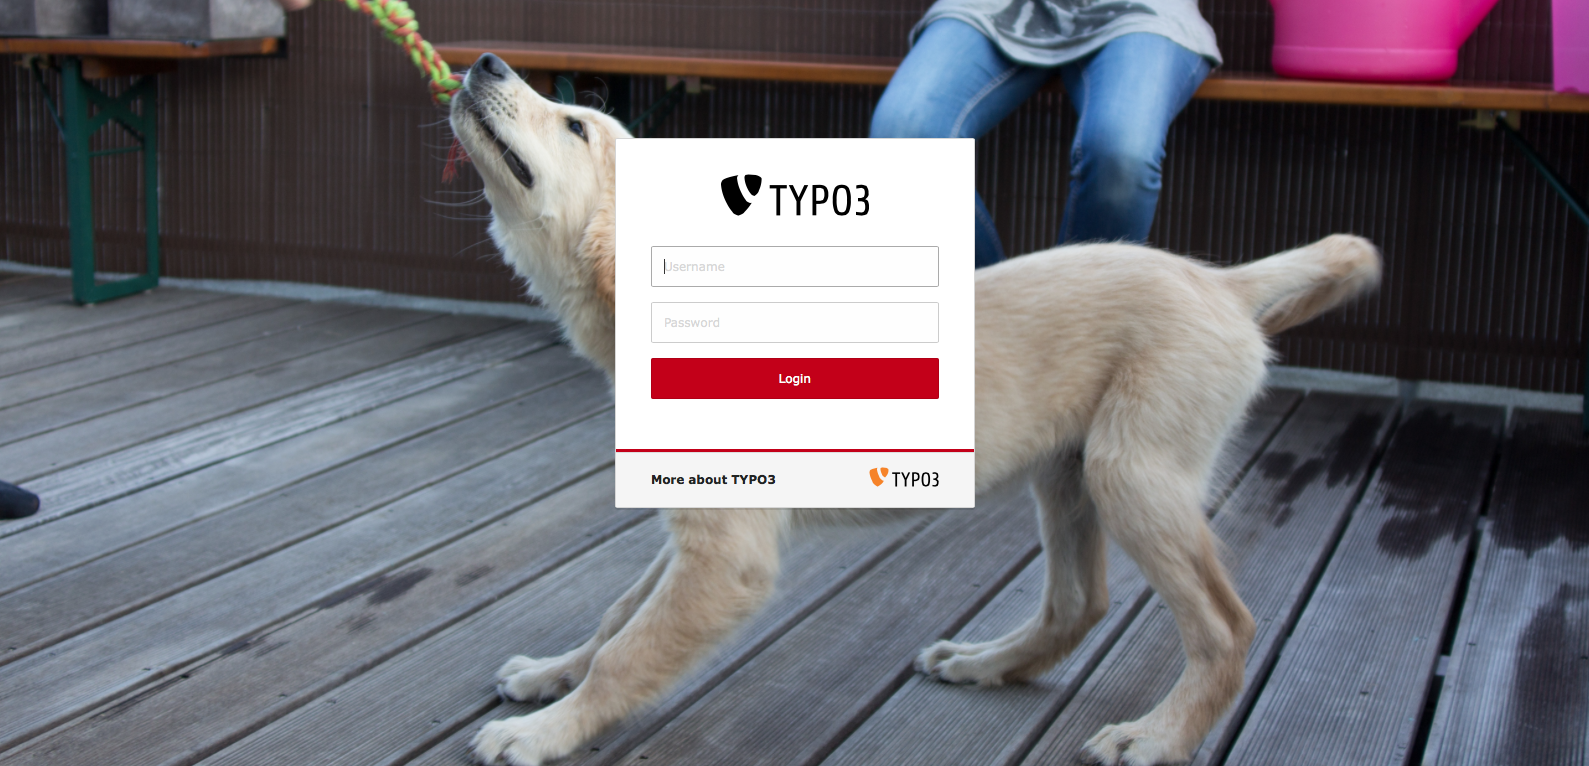
\includegraphics[width=0.75\linewidth]{BackendUserInterface/Login.png}
	\end{figure}

\end{frame}

% ------------------------------------------------------------------------------
% LTXE-SLIDE-START
% LTXE-SLIDE-UID:		fb5d330d-c220cabc-cafa031f-580864a0
% LTXE-SLIDE-ORIGIN:	e2e353ae-3b2b5c00-0cd7c57d-d97d22c9 English
% LTXE-SLIDE-TITLE:		Add image cropping
% LTXE-SLIDE-REFERENCE:	Feature-65584-AddImageCropping.rst
% ------------------------------------------------------------------------------
\begin{frame}[fragile]
	\frametitle{Interfaccia utente Backend}
	\framesubtitle{Manipolazione immagini: Cropping}

	Una funzionalità di manipolazione immagini permette all'editore di ritagliare le immagini nel backend.
	Questa funzione deve essere attivata esplicitamente per gli utenti di BE ("Exclude Fields"):

	\begin{figure}
		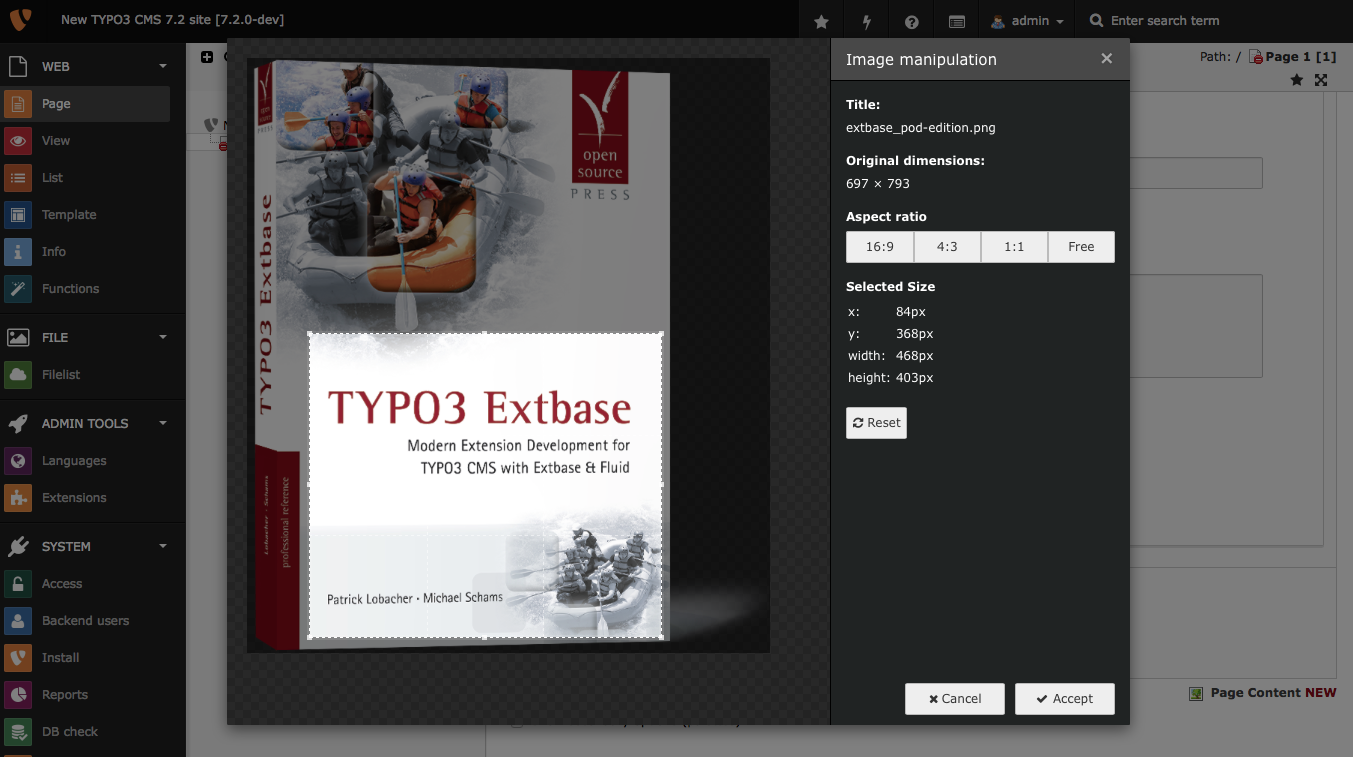
\includegraphics[width=0.7\linewidth]{BackendUserInterface/ImageCropping.png}
	\end{figure}

\end{frame}

% ------------------------------------------------------------------------------
% LTXE-SLIDE-START
% LTXE-SLIDE-UID:		21a9a7c2-0753ce0e-f3c668d8-cb2471a4
% LTXE-SLIDE-ORIGIN:	301dfea9-d2debf3e-dcaa7bcd-205e5990 English
% LTXE-SLIDE-TITLE:		Add backend user groups to backend user module
% LTXE-SLIDE-REFERENCE:	Feature-64686-AddBackendUserGroupsToBackendUserModule.rst
% ------------------------------------------------------------------------------
\begin{frame}[fragile]
	\frametitle{Interfaccia utente Backend}
	\framesubtitle{Gruppi di utenti di Backend}

	I gruppi di utenti del Backend possono essere gestiti in un sottomodulo del modulo "Utenti di Backend":

	\begin{figure}
		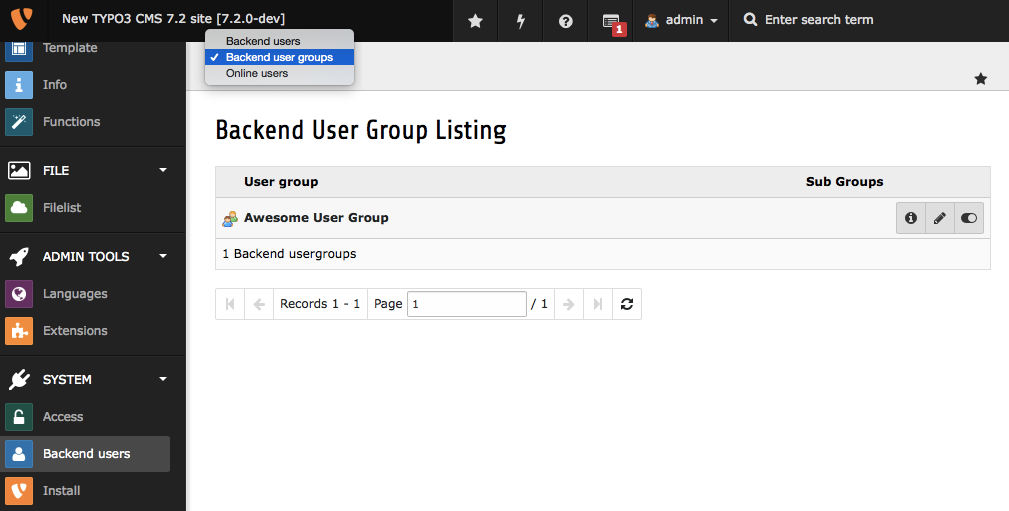
\includegraphics[width=0.70\linewidth]{BackendUserInterface/UserGroups.png}
	\end{figure}

\end{frame}

% ------------------------------------------------------------------------------
% LTXE-SLIDE-START
% LTXE-SLIDE-UID:		4dacae70-b095c549-96609323-a04e731c
% LTXE-SLIDE-ORIGIN:	daa83c1e-08d2716b-de74cbda-42361551 English
% LTXE-SLIDE-TITLE:		Extension Manager: Disable automatic installation
% LTXE-SLIDE-REFERENCE:	Feature-50501-DisableAutomaticExtInstallation.rst
% ------------------------------------------------------------------------------
\begin{frame}[fragile]
	\frametitle{Interfaccia utente Backend}
	\framesubtitle{Disabilitare installazione automatica delle estensioni}

	L'amministratore può configurare l'Extension Manager a non installare subito le
	estensioni scaricate:

	\begin{figure}
		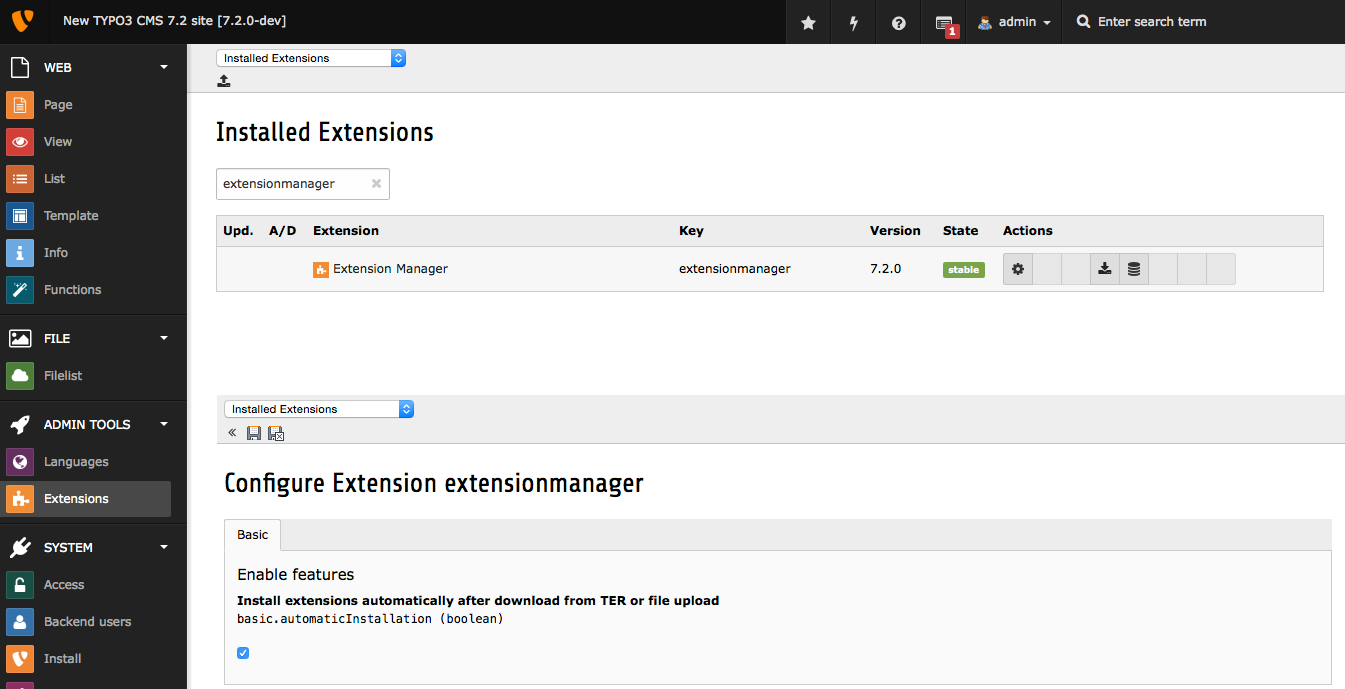
\includegraphics[width=0.70\linewidth]{BackendUserInterface/ExtManager.png}
	\end{figure}

\end{frame}

% ------------------------------------------------------------------------------
% LTXE-SLIDE-START
% LTXE-SLIDE-UID:		a50f9c9e-a0575418-18d7bf7c-60a808a0
% LTXE-SLIDE-ORIGIN:	20769920-da9df227-c3b527b9-9a23bac1 English
% LTXE-SLIDE-TITLE:		Show remaining characters below text fields
% LTXE-SLIDE-REFERENCE:	Feature-66029-ShowRemainingCharactersBelowTextFields.rst
% ------------------------------------------------------------------------------
\begin{frame}[fragile]
	\frametitle{Interfaccia utente Backend}
	\framesubtitle{Caratteri rimanenti nel campo Testo}

	Il numero di caratteri rimanenti è visualizzato sotto il campo di inserimento testo:

	\begin{figure}
		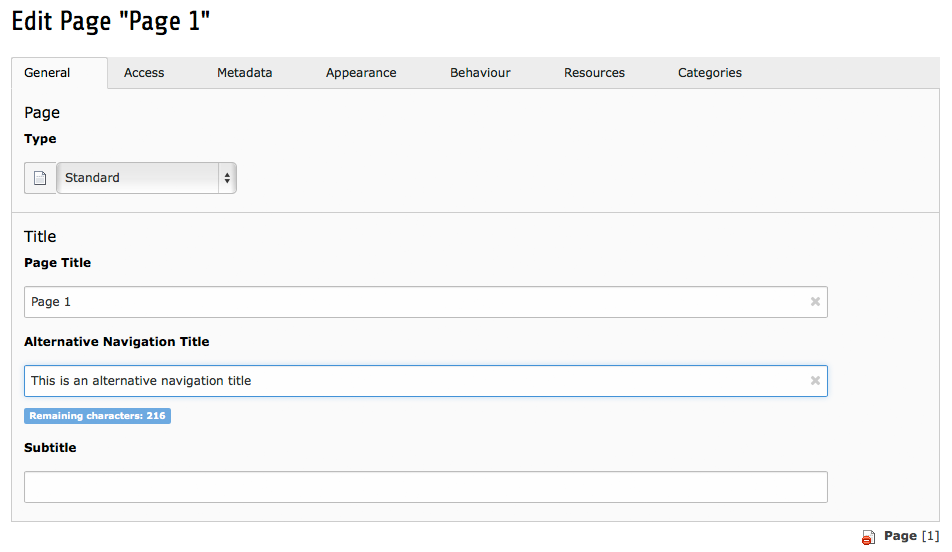
\includegraphics[width=0.70\linewidth]{BackendUserInterface/RemainingCharacters.png}
	\end{figure}

\end{frame}

% ------------------------------------------------------------------------------
% LTXE-SLIDE-START
% LTXE-SLIDE-UID:		c3314ee2-46aad046-00d0fbfa-8df063e1
% LTXE-SLIDE-ORIGIN:	ff760b86-9d6b1ecd-d0e98565-f23c51f0 English
% LTXE-SLIDE-TITLE:		Show confirm message on closing an editform with unsaved changes
% LTXE-SLIDE-REFERENCE:	Feature-65996-AddConfirmationOnCloseEditformWithUnsavedChanges.rst
% ------------------------------------------------------------------------------
\begin{frame}[fragile]
	\frametitle{Interfaccia utente Backend}
	\framesubtitle{Conferma modifiche non salvate}

	Un nuovo messaggio di avvertimento è mostrato all'editore per evitare la perdita di modiche non salvate:

	\begin{figure}
		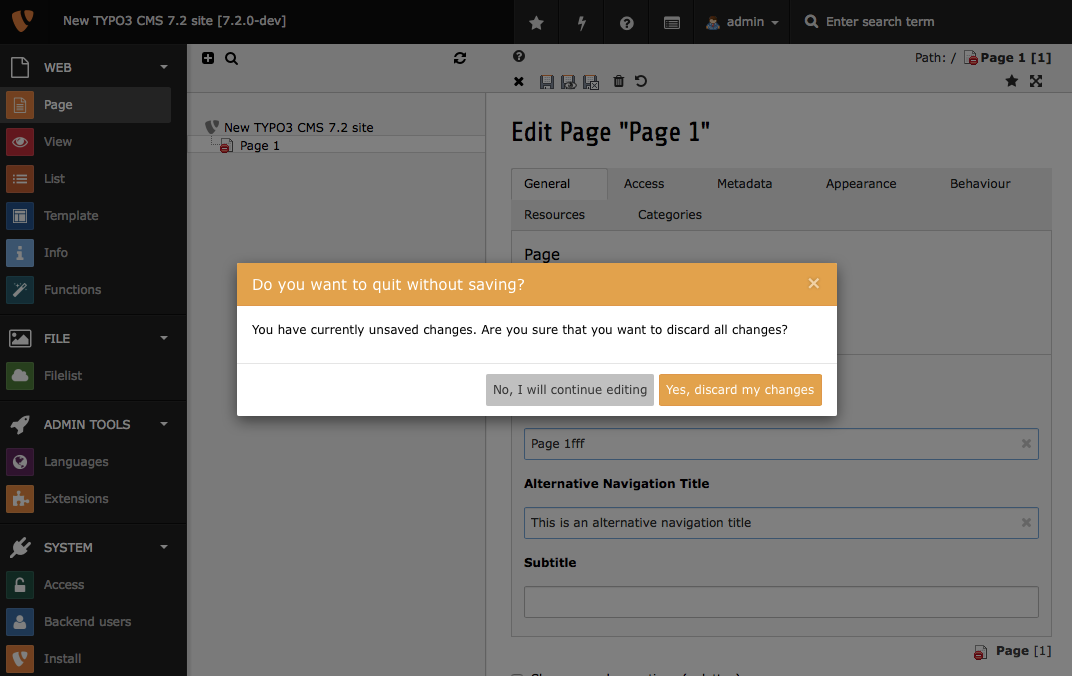
\includegraphics[width=0.65\linewidth]{BackendUserInterface/ClosingDialog.png}
	\end{figure}

\end{frame}

% ------------------------------------------------------------------------------
% LTXE-SLIDE-START
% LTXE-SLIDE-UID:		e9ed3f5d-35a2b3da-214245a6-be744f5a
% LTXE-SLIDE-ORIGIN:	6ac9a35e-46541895-7509263e-28fb799f English
% LTXE-SLIDE-TITLE:		System Information Dropdown
% LTXE-SLIDE-REFERENCE:	Feature-65767-SystemInformationDropdown.rst
% ------------------------------------------------------------------------------
\begin{frame}[fragile]
	\frametitle{Interfaccia utente Backend}
	\framesubtitle{Tendina con informazioni di sistema}

	Un menu a tendina mostra diverse informazioni sul sistema TYPO3 installato.
	I dati di questo box possono essere integrati:\newline
	\small(vedi il capitolo "Modifiche rilevanti" per maggiori dettagli)\normalsize

	\begin{figure}
		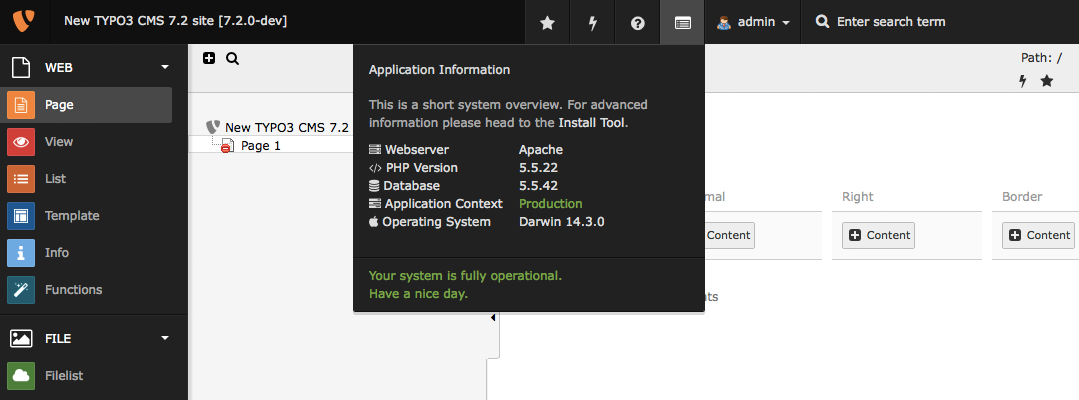
\includegraphics[width=0.85\linewidth]{BackendUserInterface/SystemInformation.png}
	\end{figure}

\end{frame}

% ------------------------------------------------------------------------------
% LTXE-SLIDE-START
% LTXE-SLIDE-UID:		f8f9b126-950be155-84e42bf9-217b5f92
% LTXE-SLIDE-ORIGIN:	79a2ee0c-3439d600-08990adb-6bed8c19 English
% LTXE-SLIDE-TITLE:		Ask for old password when changing
% LTXE-SLIDE-REFERENCE:	commit bf6f5226eb6cb441bb53657a88ef42f1cdb5155f
% ------------------------------------------------------------------------------
\begin{frame}[fragile]
	\frametitle{Interfaccia utente Backend}
	\framesubtitle{Cambio Password}

	Gli utenti di Backend devono inserire la password attuale (vecchia) per poter inserire
	una nuova password:

	\begin{figure}
		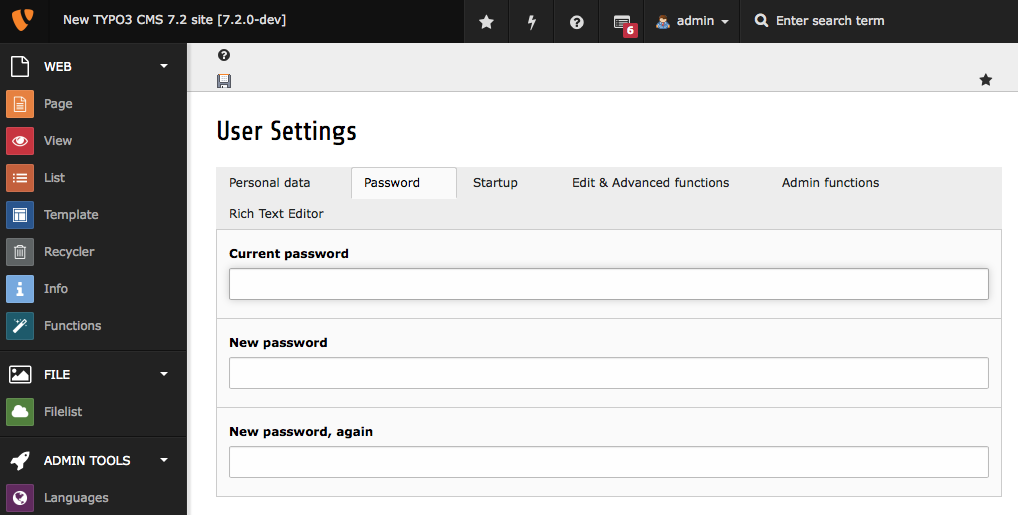
\includegraphics[width=0.7\linewidth]{BackendUserInterface/Password.png}
	\end{figure}

\end{frame}

% ------------------------------------------------------------------------------
% LTXE-SLIDE-START
% LTXE-SLIDE-UID:		18c5551c-ed17e331-dbbacc7d-d6fdfa6b
% LTXE-SLIDE-ORIGIN:	7725bce9-e606f055-bf2e7b4a-e870fe2a English
% LTXE-SLIDE-TITLE:		Add icon for "Show Content From Page"
% LTXE-SLIDE-REFERENCE:	commit f8aa3eea9aed97a901ef0c3e7c650e1218839596
% ------------------------------------------------------------------------------
\begin{frame}[fragile]
	\frametitle{Interfaccia utente Backend}
	\framesubtitle{Icona pagina per "Mostra contenuti di altra pagina"}

	Una nuova icona di pagina nell'albero delle pagine indica che la pagina mostra i contenuti di un altra pagina:

	\begin{figure}
		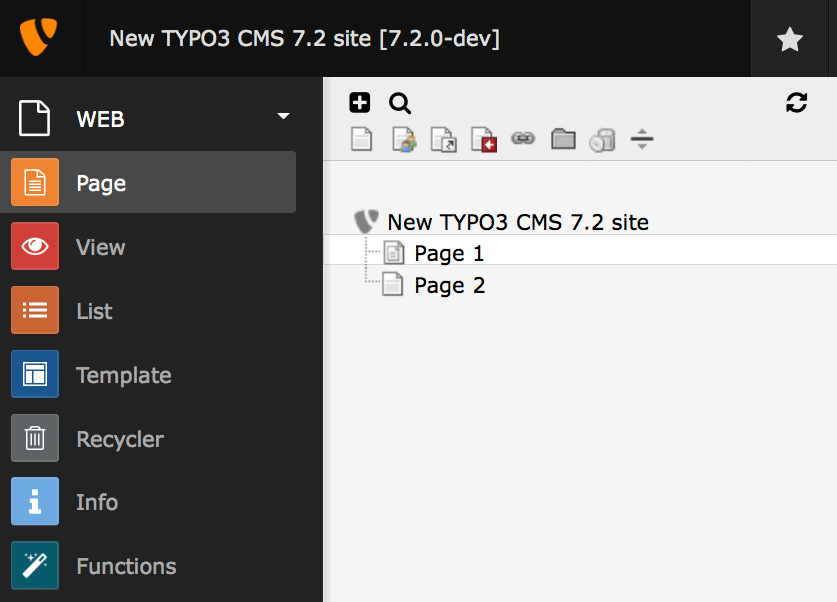
\includegraphics[width=0.45\linewidth]{BackendUserInterface/ShowContent.png}
	\end{figure}

\end{frame}

% ------------------------------------------------------------------------------
% LTXE-SLIDE-START
% LTXE-SLIDE-UID:		60c81bad-c3f4fb28-d11cbc75-3e10abeb
% LTXE-SLIDE-ORIGIN:	5ac2de45-9be12bf9-1c326192-602839fb English
% LTXE-SLIDE-TITLE:		Extension Manager: Choose version for update
% LTXE-SLIDE-REFERENCE:	commit a26396a4530b530744ec8b36c5fb5606789a6739
% ------------------------------------------------------------------------------
\begin{frame}[fragile]
	\frametitle{Interfaccia utente Backend}
	\framesubtitle{Aggiornamento estensioni}

	Quando si aggiorna un estensione, è possibile scegliere il numero di versione da installare:

	\begin{figure}
		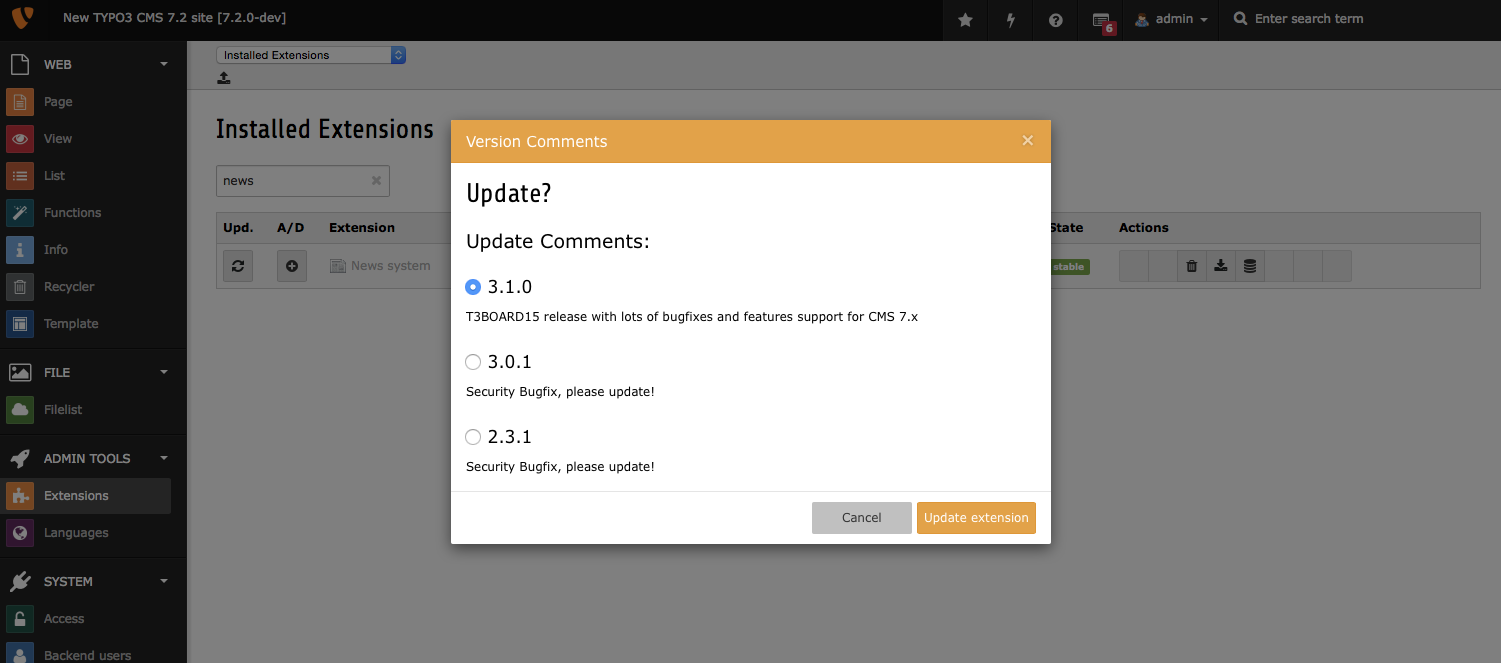
\includegraphics[width=0.75\linewidth]{BackendUserInterface/Update.png}
	\end{figure}

\end{frame}

% ------------------------------------------------------------------------------
% LTXE-SLIDE-START
% LTXE-SLIDE-UID:		6bc1a460-29c61401-62097e4a-bccfcd90
% LTXE-SLIDE-ORIGIN:	f6be31f7-155d676c-0e551545-3fc89e89 English
% LTXE-SLIDE-TITLE:		Add scheduler task to remove deleted records
% LTXE-SLIDE-REFERENCE:	Feature-32651-AddSchedulerTaskToRemoveDeletedRecords.rst
% ------------------------------------------------------------------------------
\begin{frame}[fragile]
	\frametitle{Interfaccia utente Backend}
	\framesubtitle{Attività Recycler}

	Una nuova attività dello scheduler per l'estensione di sistema \texttt{recycler} rimuove i
	record cancellati dalle tabelle di contenuti nel database. L'età massima e le tabelle coinvolte
	sono configurabili nelle impostazioni dell'attività.
	Questo può essere applicato anche ai file, se sono referenziati agli elementi di contenuto.

	\begin{figure}
		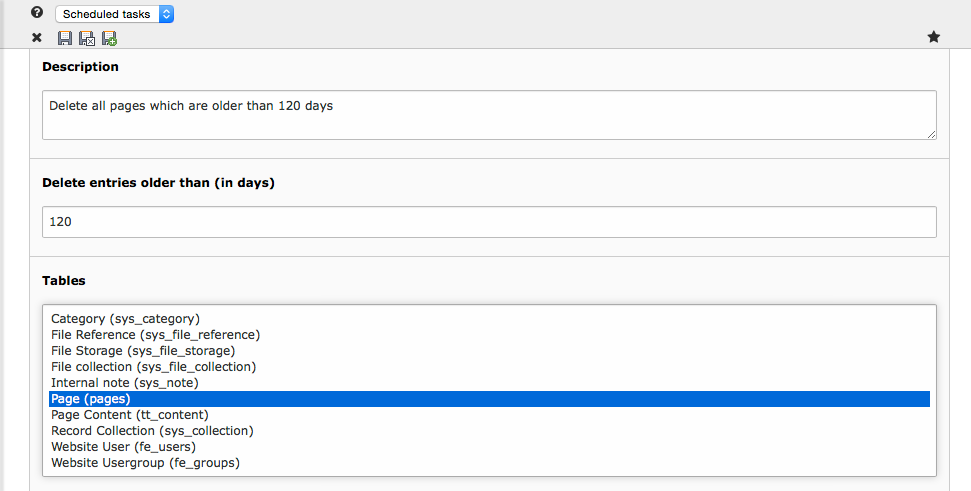
\includegraphics[width=0.60\linewidth]{BackendUserInterface/RecyclerTask.png}
	\end{figure}

\end{frame}

% ------------------------------------------------------------------------------
